\chapter{Non-Resonance 7 TeV Analysis}
\label{ch:7tev}

This chapter looks at the non-resonant analysis done within ATLAS on 2011 data and was a measurement made prior to the other analysis presented in this thesis. The author made a major contribution to this analysis working on the dielectron search channel and pushing it through to publication \cite{PhysRevD.87.015010}. 
The 7 TeV analysis major differences come from not including the angular search in $\cos{\theta^{*}}$ and looking at only the LL CI formalism and GRW ADD formalism. 
Background simulation differs slightly with different generators used and the explicit change from the QCD and W+jets background to the more inclusive multijets \& and W+jets obtained fully via a data driven method. The event selection also differs between the two analyses with the optimisation of the isolation selection and updated shower shape selection in the 8 TeV analysis. The big change is the addition of the angular analysis with respect to $\cos\theta^{*}$ introducing the opposite sign requirement and changing the search bins used in the Bayesian analysis. A slightly smaller list of systematic errors were included in this analysis compared to the 8 TeV one.
Below is an overview of each part of this analysis with comparisons between this and the main analysis spoken of in this thesis.




%comparisons between analyses


\section{Data and Background Processes}

\subsection*{Data}
	All data used in this analysis is taken from the LHC 2011 $\sqrt{s} = 7 TeV$ proton-proton collision data of which ATLAS recorded $4.9 fb^{-1}$ of electron candidate data. Data was collected with stable LHC beams and a fully operational inner detector and calorimeter each being important in the identification of good electron candidates.

\subsection*{Background}
	%The main background the non resonant signal in the electron channel is Drell-Yan (DY) $\rightarrow~ee$ production mediated by a photon or the Z boson. However there are other small contributions from $t\bar{t}$, diboson, W + jets and QCD production. $t\bar{t}$ background consists of events with $t\bar{t}$ production decaying to amongst other things two electrons. Diboson background can involve either an event producing two W bosons, two Z boson or one W and one Z boson in which two electrons also exist in the final decay state. Both these productions can result in two electrons with a large combined invariant mass which could mimic signal production. W + jets production can result in an electron and a jet faking an electron left in the final state, while QCD refers to events where two jets fake electrons. These all combine to form the background sample.

	The background precess are the same between analyses with slight differences in the MC generators used. The bigger difference however are the comparisons between the W+jets and QCD backgrounds used in this analysis with the multijet \& W+jets background used in the 8 TeV analysis. This difference is mainly naming differences but here the background is produced through a combination of a MC sample and a data driven method while the 8 TeV analysis uses only a data driven method. 

	Standard Model Drell-Yan was simulated by the leading-order (LO) PYTHIA 6 \cite{} Monte Carlo (MC) event generator. This method was used to generate a $Z\rightarrow~ee$ sample for the low dielectron invariant mass region ($m_{ee} < 120 GeV$) and a $DY\rightarrow~ee$ mass binned sample for the invariant high mass ($m_{ee} > 120 GeV$) to keep high statistics at high invariant mass. Similarly to the 8 TeV analysis K-factors are used here to weight from the LO prediction up a nnlo prediction. Four other samples are included to produce the background estimate, these are: $t\bar{t}$, produced with MC@NLO \cite{}; diboson, WW, WZ and ZZ decays produced with HERWIG \cite{}; W+jets, produced with ALPGEN \cite{}, JIMMY \cite{} and HERWIG \cite{}; and QCD, produced using a data driven method.

\subsection*{Signal} 

	Five benchmarks for the value of $\Lambda$ where chosen for the CI signal samples for both constructive and destructive interference. Like the DY these were also produced with LO PYTHIA containing both the pure DY contribution as well as the interference and pure CI components. Samples where produced above dilepton invariant mass of 120 GeV to increase statistics above the Z boson peak where new physics would appear. 

	ADD samples were generated using SHERPA \cite{} at leading order with 4 values of M$_{s}$ produced. Samples were again produced above dilepton invariant mass of 120 GeV. 

	% \begin{table}[h!]
	% \centering % centering table
	% \begin{tabular}{l ccc} % creating eight columns
	% \hline\hline \\[-2ex] %inserting double-line
	% $m_{ee}$ [GeV] & 120-300 & 300-600 & $\geq 600$ \\ [0.2ex]
	% \hline  \\[-2ex] % inserts single-line
	% $\Lambda^{-} = 3$ TeV & 9.8583 & 0.96765 & 0.77563 \\ 
	% $\Lambda^{-} = 4$ TeV & 9.3400 & 0.50510 & 0.26647 \\ 
	% $\Lambda^{-} = 5$ TeV & 9.0960 & 0.36935 & 0.12733 \\  
	% $\Lambda^{-} = 7$ TeV & 8.9686 & 0.28401 & 0.048406 \\  
	% $\Lambda^{-} = 12$ TeV & 8.9037 & 0.24774 & 0.021028 \\ 
	% \hline  \\[-2ex] % inserts single-line
	% $\Lambda^{+} = 3$ TeV & 8.9018 & 0.65247 & 0.66034 \\ 
	% $\Lambda^{+} = 4$ TeV & 8.8756 & 0.33164 & 0.20668 \\  
	% $\Lambda^{+} = 5$ TeV & 8.7362 & 0.25646 & 0.085934 \\ 
	% $\Lambda^{+} = 7$ TeV & 8.8101 & 0.22656 & 0.028772 \\ 
	% $\Lambda^{+} = 12$ TeV & 8.9045 & 0.22774 & 0.014418 \\ 
	% \hline\hline  \\ %[0.2ex] %inserting double-line
	% \end{tabular}
	% \caption{Table of CI sample cross sections [$pb^{-1}$].} %title of the table
	% \label{tab:CIyeilds}
	% \end{table}

	Corrections are applied to all MC samples. A correction handling event pile-up is applied on an event by event basis as well as QCD and Electroweak K-factor corrections applied as a function of invariant mass to the signal samples and SM DY samples. The K-factors applied to DY scales the original LO predictions using the MRST2007LO** \cite{} PDF to the MSTW2008NNLO \cite{} PDF. These corrections did not change in method between the 7 and 8 TeV analyses and are discussed in more detail in section \ref{sec:correc}.



\section{Electron Identification and Selection}

	The selection of electron candidates for the CI and ADD analysis can be split in three main parts, selection of a good event, selection of a set of good electrons and selection of a good dielectron pair.\\

	{\bf Event Selection}
	\begin{itemize}
	\item Each event is required to contain at least one reconstructed primary vertex with more than 2 charged tracks traceable to it.
	\item Event is required have passed the chosen unprescaled electron trigger (EF\_g20\_loose).
	\end{itemize}

	{\bf Electron Selection}
	\begin{itemize}
	\item Each electron is required to have a transverse momentum ($p_{T}$) greater than 25 GeV.
	\item Electron $|\eta| < 2.47$ and not lie within the detector crack region $1.37 \leq |\eta| \leq 1.52$ due to a decreased energy resolution.
	%\item Electron must not be 
	\item Electrons are required to pass identification criteria on the transverse shower shape, the longitudinal leakage into the hadronic calorimeter, and the association to an inner detector track, defined together as a ``medium'' electron identification.
	\item If expected electron is required to have signal in the inter most level of the tracking detector (B-layer). Used to suppress background from photon conversions.
	\end{itemize}

	{\bf Dielectron Selection}
	\begin{itemize}
	\item Selection of two highest $p_{T}$ electrons left in event.
	\item Isolation (A cone around the candidate in the calorimeter is required to have $< 7 GeV$ deposited in it) of the highest $p_{T}$ electron in the event is required to suppress QCD jet background. 
	\item Dielectron invariant mass (m$_{ee}$) is required to be greater than or equal 70 GeV.
	\end{itemize}

	Between the two analyses a few difference appear in the the event selection. The trigger used is different in each case as the lowest threshold unprescaled trigger that is available is used for each data set. Transverse momentum requirements have then changed in accordance with the thresholds of the triggers as well as the increase in the invariant mass requirement for the same reason. The identification of a ``medium'' electron was updated between the two analyses with the 8 TeV version also including the expected signal in the tracking detector B-layer as a requirement. The isolation requirement underwent an optimisation between the two analyses detailed in section \ref{sec:iso}. The final difference is the lack of opposite sign requirement in this analysis.

	These remaining candidates are then the results. The signal region is defined as $m_{ee} > 150$ GeV while the $70 \leq m_{ee} \leq 150$ GeV region is used as a control region.

	\begin{table}[h!]
	\centering % centering table
	\begin{tabular}{l cccccc} % creating eight columns
	\hline\hline \\[-2ex] %inserting double-line
	$m_{ee}$ [GeV] & 70-110 & 110-200 & 200-400 \\  [0.2ex]
	\hline  \\[-2ex] % inserts single-line
	DY & 1231053.7 $\pm$ 1109.5 & 26756.7 $\pm$ 163.6 & 2964.0 $\pm$ 54.4 \\ 
	$t\bar{t}$ & 879.6 $\pm$ 29.7 & 1008.8 $\pm$ 31.8 & 315.8 $\pm$ 17.8 \\ 
	Dibosons & 1827.1 $\pm$ 42.7 & 415.4 $\pm$ 20.4 & 146.6 $\pm$ 12.1 \\ 
	QCD + W+jets & 2885.7 $\pm$ 53.7 & 1892.0 $\pm$ 43.5 & 510.5 $\pm$ 22.6 \\ [0.2ex]
	\hline  \\[-2ex] % inserts single-line
	Total & 1236646.0 $\pm$ 1112.0 & 30072.9 $\pm$ 173.4 & 3936.9 $\pm$ 62.7 \\ [0.2ex]
	\hline  \\[-2ex] % inserts single-line
	Data & 1236646 & 29816 & 4026 \\ [0.2ex]
	\hline\hline  \\ %[0.2ex] %inserting double-line
	\end{tabular}
	\begin{tabular}{ccc} % creating eight columns
	\hline\hline \\[-2ex] %inserting double-line
	400-800 & 800-1200 & 1200-3000 \\  [0.2ex]
	\hline  \\[-2ex] % inserts single-line
	266.0 $\pm$ 16.3 & 12.2 $\pm$ 3.5 & 1.5 $\pm$ 1.2 \\ 
	20.5 $\pm$ 4.5 & 0.3 $\pm$ 0.6 & 0.0 $\pm$ 0.2 \\ 
	16.5 $\pm$ 4.1 & 0.9 $\pm$ 0.9 & 0.1 $\pm$ 0.3 \\ 
	49.5 $\pm$ 7.0 & 2.0 $\pm$ 1.4 & 0.3 $\pm$ 0.5 \\ [0.2ex]
	\hline  \\[-2ex] % inserts single-line
	352.4 $\pm$ 18.8 & 15.4 $\pm$ 3.9 & 1.9 $\pm$ 1.4 \\ [0.2ex]
	\hline  \\[-2ex] % inserts single-line
	358 & 17 & 3 \\ [0.2ex]
	\hline\hline  \\ %[0.2ex] %inserting double-line
	\end{tabular}
	\caption{Table of data yeild compared to background MC scaled to luminosity of data. Errors shown are statistical only.} %title of the table
	\label{tab:dataMCyields}
	\end{table}



\subsection{Data and Background Comparison}

	Table \ref{tab:dataMCyields} shows the number of data events remaining after selection of dielectron candidates compared to the total background prediction with all individual background components also shown. The simulated MC samples also undergo a scaling factor to scale within the Z boson peak. This scale factor works the same as in the 8 TeV analysis only within the slightly more limited range $70 \leq m_{ee} \leq 110$ GeV. As can be seen the background prediction matches very closely to data within the statistical errors shown.


	\begin{figure}[h!]
	\centering
	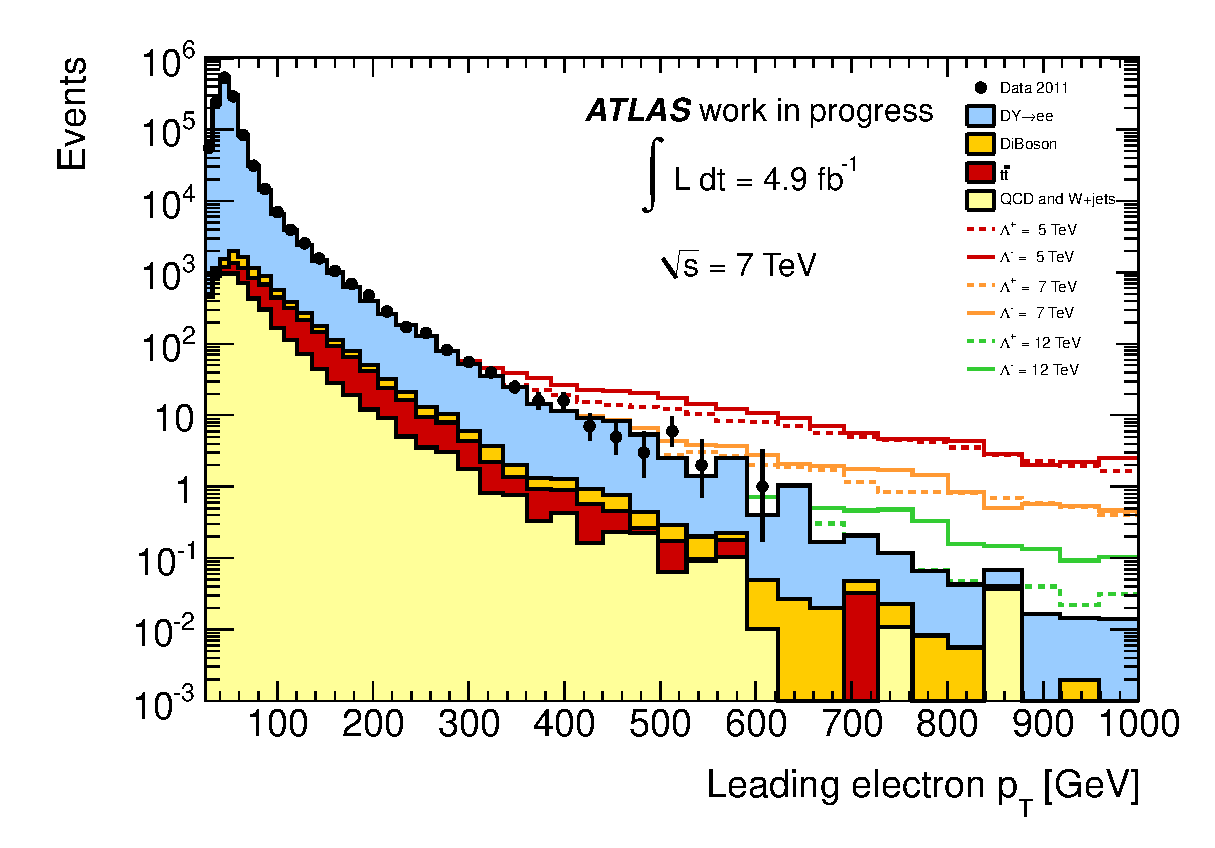
\includegraphics[width=0.49\linewidth]{images/lead_pT.eps}
	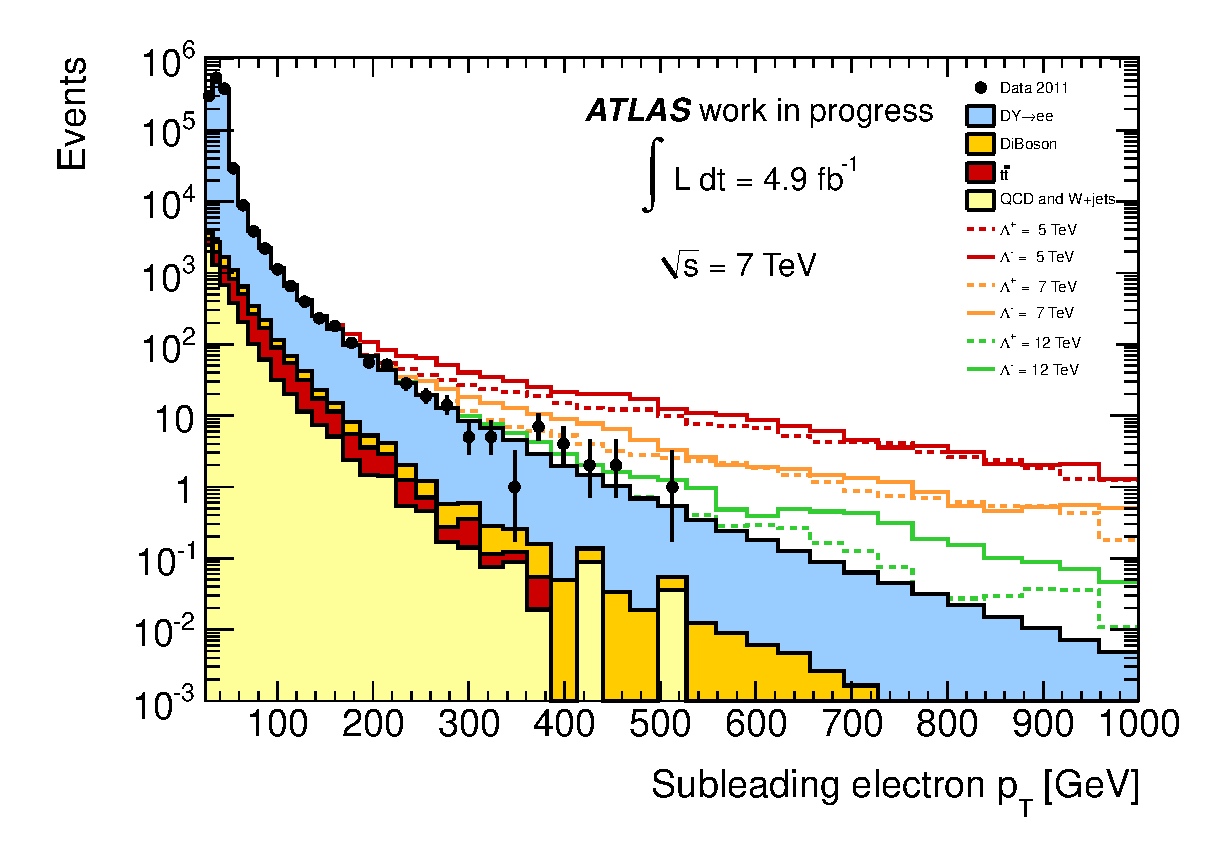
\includegraphics[width=0.49\linewidth]{images/sub_pT.eps}
	\caption{$p_{T}$ distribution of the leading (left) and subleading (right) electrons showing data, MC background and example CI signal samples compared to data.}
	\label{fig:CIpT}
	\end{figure}

	\begin{figure}[h!]
	\centering
	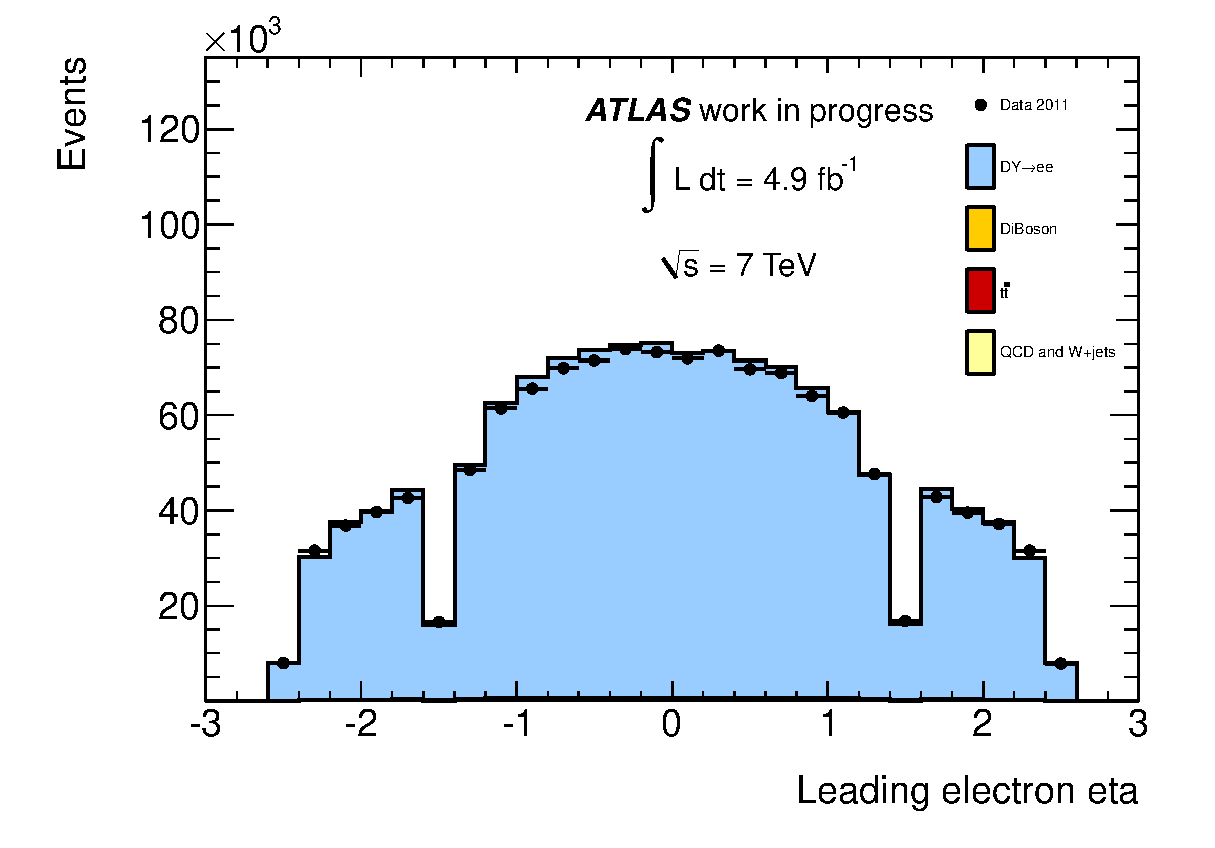
\includegraphics[width=0.49\linewidth]{images/lead_eta.eps}
	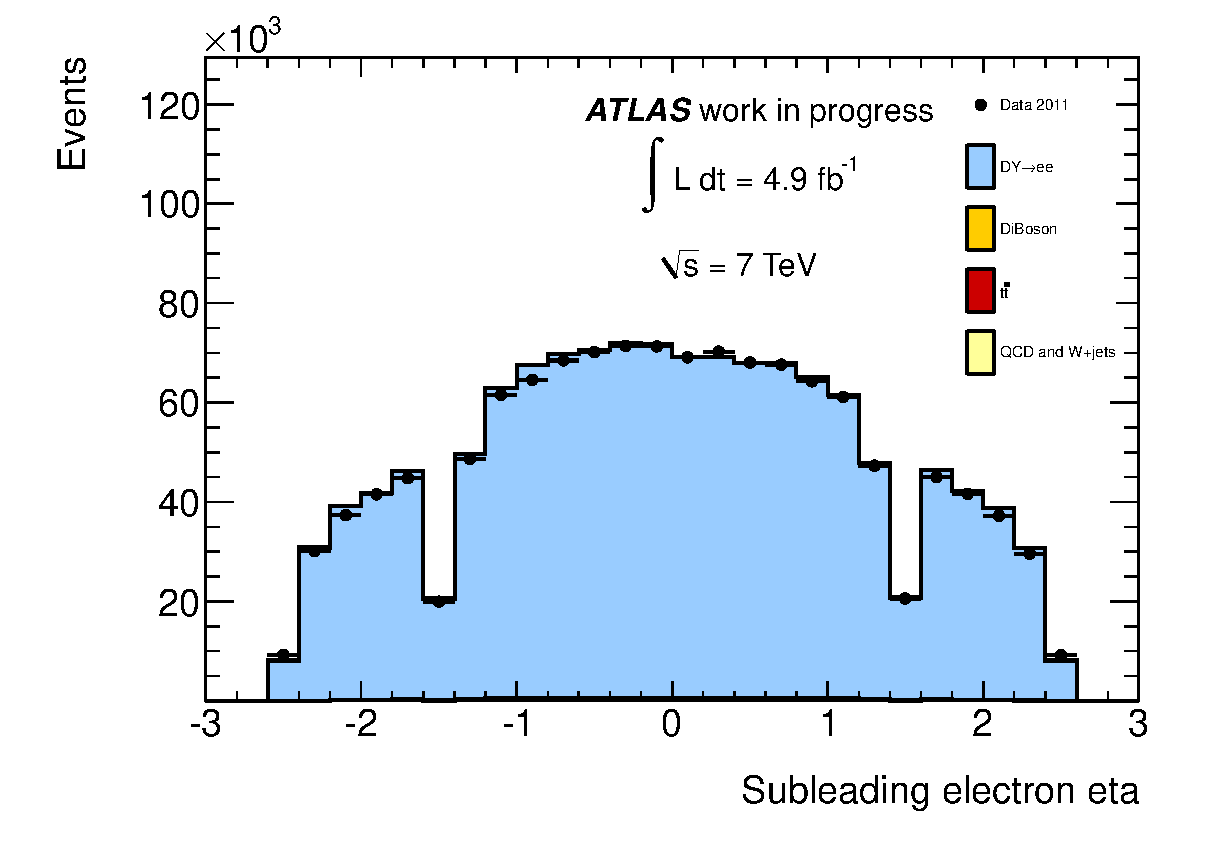
\includegraphics[width=0.49\linewidth]{images/sub_eta.eps}
	\caption{$\eta$ distribution of the leading (left) and subleading (right) electrons showing data, MC background compared to data.}
	\label{fig:eta}
	\end{figure}

	Control plots were produced to display that the distributions were behaving as predicted such as the $p_{T}$ (Fig. \ref{fig:CIpT}) and the $\eta$ (Fig. \ref{fig:eta}) distributions.





\subsection{New Physics Signal Expectation}
%(analysis method)

	\begin{table}[h!]
	\small 
	\centering % centering table
	\begin{tabular}{l ccccc} % creating eight columns
	\hline\hline \\[-2ex] %inserting double-line
	$m_{ee}$ [GeV] & 110-200 & 200-400 & 400-800 & 800-1200 & 1200-3000 \\ [0.2ex]
	\hline  \\[-2ex] % inserts single-line
	$\Lambda^{-} = 3$ TeV & 18790.8 $\pm$ 137.1 & 5022.4 $\pm$ 70.9 & 2766.3 $\pm$ 52.6 & 1089.2 $\pm$ 33.0 & 673.3 $\pm$ 25.9 \\ 
	$\Lambda^{-} = 4$ TeV & 18212.5 $\pm$ 135.0 & 3707.1 $\pm$ 60.9 & 1102.5 $\pm$ 33.2 & 356.9 $\pm$ 18.9 & 214.3 $\pm$ 14.6 \\ 
	$\Lambda^{-} = 5$ TeV & 17821.5 $\pm$ 133.5 & 3310.5 $\pm$ 57.5 & 653.1 $\pm$ 25.6 & 160.6 $\pm$ 12.7 & 97.7 $\pm$ 9.9 \\ 
	$\Lambda^{-} = 7$ TeV & 17711.1 $\pm$ 133.1 & 3018.8 $\pm$ 54.9 & 385.0 $\pm$ 19.6 & 56.1 $\pm$ 7.5 & 26.5 $\pm$ 5.1 \\ 
	$\Lambda^{-} = 12$ TeV & 17693.4 $\pm$ 133.0 & 2992.7 $\pm$ 54.7 & 296.5 $\pm$ 17.2 & 20.4 $\pm$ 4.5 & 5.6 $\pm$ 2.4 \\ 
	\hline  \\[-2ex] % inserts single-line
	$\Lambda^{+} = 3$ TeV & 18106.6 $\pm$ 134.6 & 4063.8 $\pm$ 63.7 & 2103.3 $\pm$ 45.9 & 918.1 $\pm$ 30.3 & 621.4 $\pm$ 24.9 \\ 
	$\Lambda^{+} = 4$ TeV & 17958.1 $\pm$ 134.0 & 3178.6 $\pm$ 56.4 & 765.6 $\pm$ 27.7 & 288.0 $\pm$ 17.0 & 194.9 $\pm$ 14.0 \\ 
	$\Lambda^{+} = 5$ TeV & 18026.6 $\pm$ 134.3 & 2895.6 $\pm$ 53.8 & 432.1 $\pm$ 20.8 & 111.4 $\pm$ 10.6 & 78.8 $\pm$ 8.9 \\ 
	$\Lambda^{+} = 7$ TeV & 17926.4 $\pm$ 133.9 & 2857.5 $\pm$ 53.5 & 278.2 $\pm$ 16.7 & 34.3 $\pm$ 5.9 & 19.1 $\pm$ 4.4 \\ 
	\hline\hline  \\ %[0.2ex] %inserting double-line
	\end{tabular}
	\caption{Table of CI signal yields for 4.9 $fb^{-1}$.} %title of the table
	\label{tab:CIyeilds}
	\end{table}

	\begin{table}[h!]
	\centering % centering table
	\begin{tabular}{l c} % creating eight columns
	\hline\hline \\[-2ex] %inserting double-line
	$m_{ee}$ [GeV] & $\geq 1300$ \\  [0.2ex]
	\hline  \\[-2ex] % inserts single-line
	$M_{S} = 1500$ GeV (GRW) & 94.8 $\pm$ 9.7 \\ 
	$M_{S} = 2000$ GeV (GRW) & 42.7 $\pm$ 6.5 \\ 
	$M_{S} = 2500$ GeV (GRW) & 11.3 $\pm$ 3.4 \\ 
	$M_{S} = 3000$ GeV (GRW) & 3.2 $\pm$ 1.8 \\ 
	\hline\hline  \\ %[0.2ex] %inserting double-line
	\end{tabular}
	\caption{Table of ADD analysis region yields for 4.9 $fb^{-1}$.} %title of the table
	\label{tab:ADDyeilds}
	\end{table}


	Tables \ref{tab:CIyeilds} and \ref{tab:ADDyeilds} show the yield from the CI and ADD MC signals used after scaling to data luminosity. The ADD yield is only shown in a single bin above 1300 GeV as the ADD statistical analysis uses only a one bin approach to set a limit of a general increase over SM background. Table \ref{tab:dataMCADDyeilds} shows the same one bin approach to the data MC comparison table.

	\begin{table}[h!]
	\centering % centering table
	\begin{tabular}{l c} % creating eight columns
	\hline\hline \\[-2ex] %inserting double-line
	$m_{ee}$ [GeV] & $\geq 1300$ \\  [0.2ex]
	\hline  \\[-2ex] % inserts single-line
	DY & 1.1 $\pm$ 1.1 \\ 
	$t\bar{t}$ & 0.0 $\pm$ 0.1 \\ 
	Dibosons & 0.1 $\pm$ 0.3 \\ 
	QCD + W+jets & 0.2 $\pm$ 0.4 \\ 
	\hline  \\[-2ex] % inserts single-line
	Total & 1.4 $\pm$ 1.2 \\ 
	\hline  \\[-2ex] % inserts single-line
	Data & 2.0 \\ 
	\hline\hline  \\ %[0.2ex] %inserting double-line
	\end{tabular}
	\caption{Table of data and MC yields for ADD analysis region.} %title of the table
	\label{tab:dataMCADDyeilds}
	\end{table}



	\begin{figure}[h!p]
	\centering
	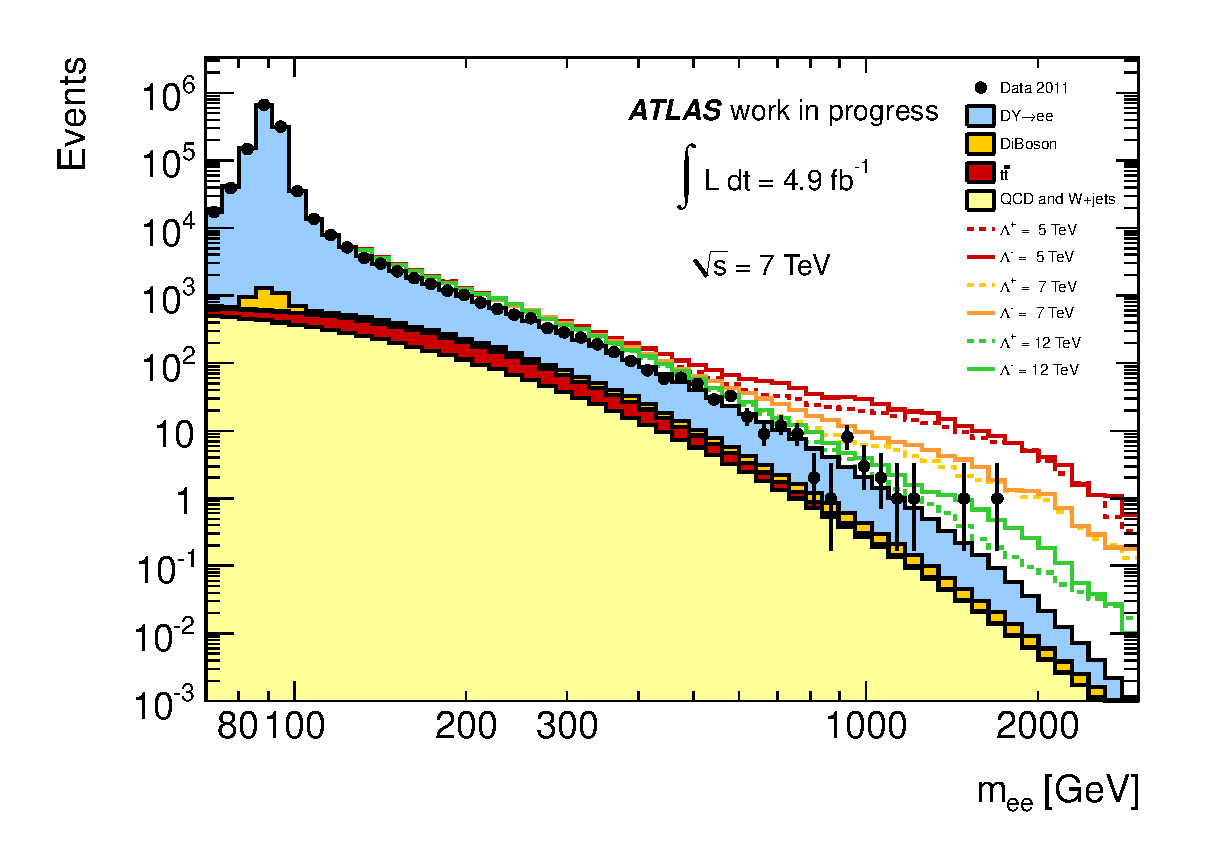
\includegraphics[width=0.9\linewidth]{images/inv_mass.eps}
	\caption{Dielectron invariant mass distribution for data and Monte Carlo simulation. Lines show expected distributions for the pressence of Contact Interactions.}
	\label{fig:CIinvMass}
	\end{figure}

	\begin{figure}[h!p]
	\centering
	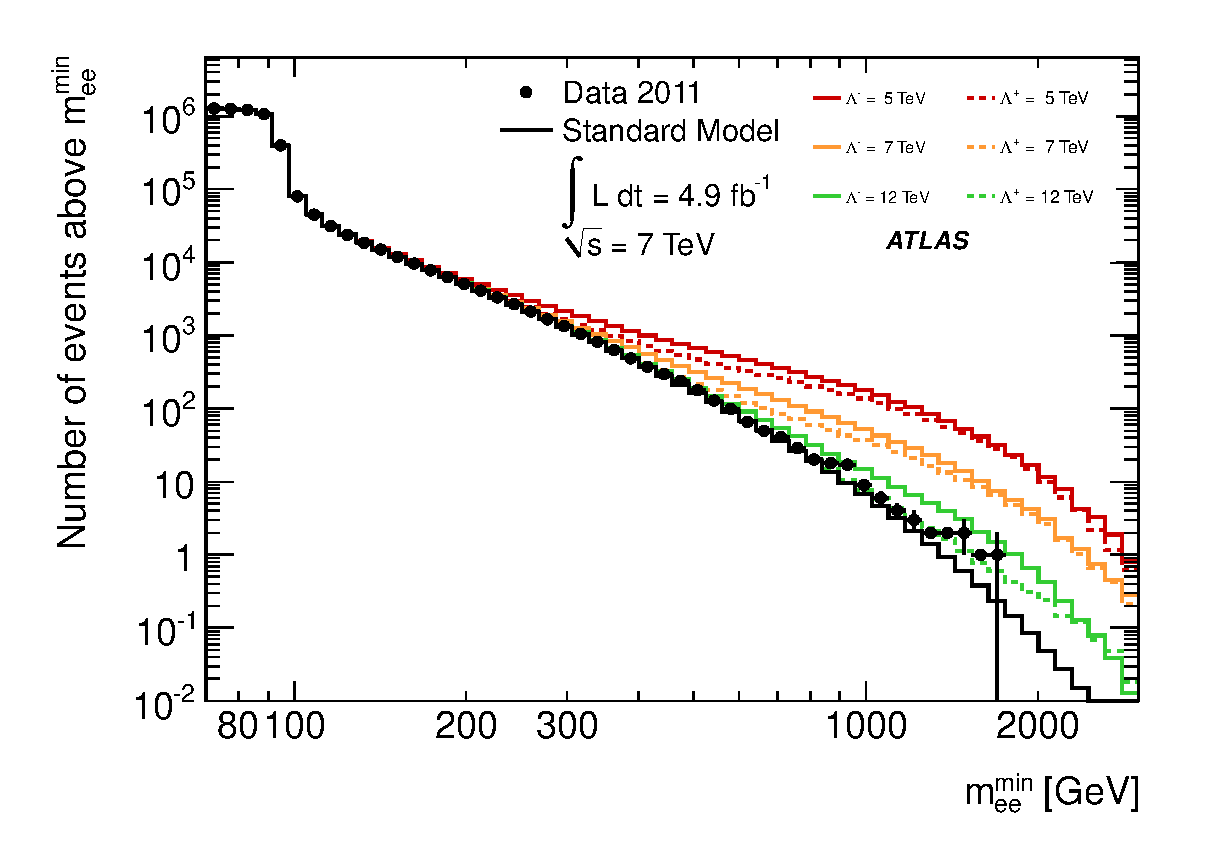
\includegraphics[width=0.9\linewidth]{images/int_inv_mass.eps}
	\caption{Dielectron intergrated invariant mass distribution for data and total background Monte Carlo simulation. Lines show expected distributions for the presence of Contact Interactions.}
	\label{fig:CIintinvMass}
	\end{figure}

	\begin{figure}[h!p]
	\centering
	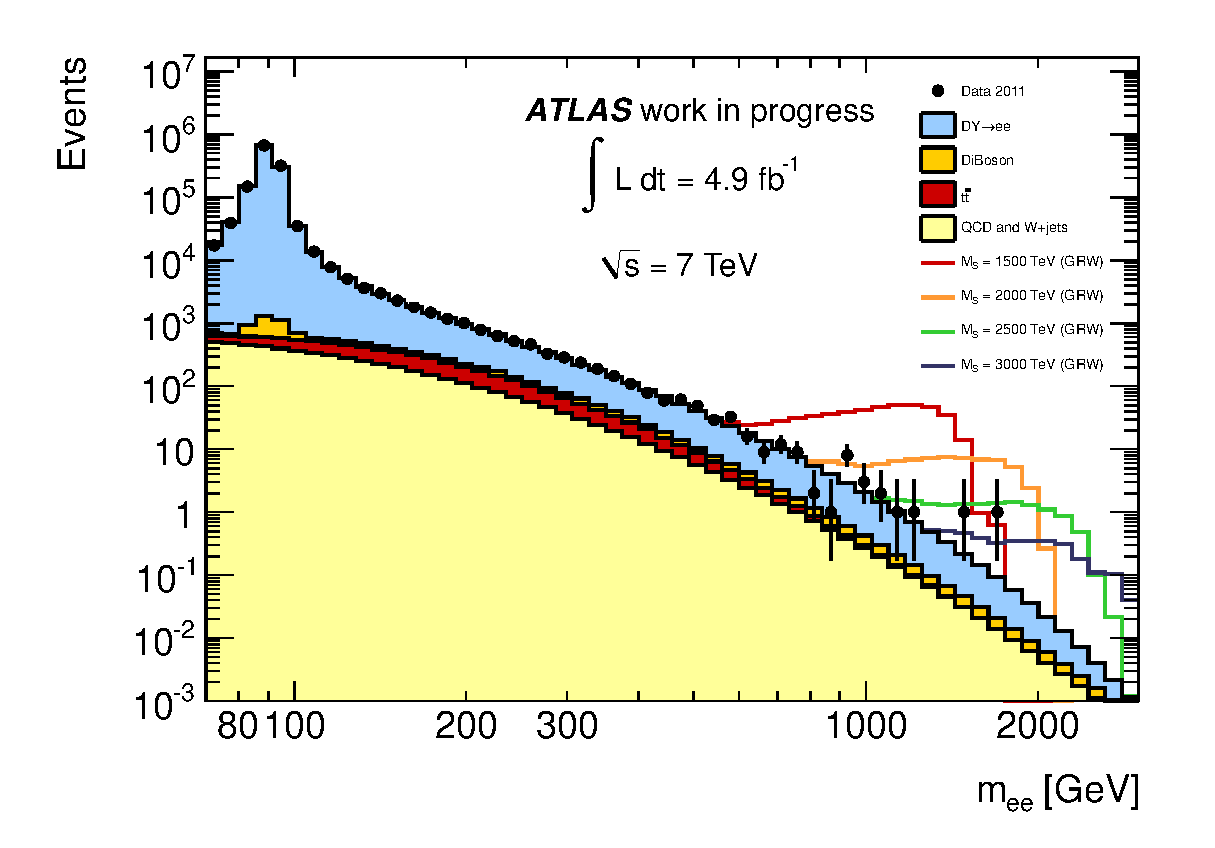
\includegraphics[width=0.9\linewidth]{images/ADD_inv_mass.eps}
	\caption{Dielectron invariant mass distribution for data and Monte Carlo simulation. Lines show expected distributions for the pressence of ADD.}
	\label{fig:ADDinvMass}
	\end{figure}

	\begin{figure}[h!p]
	\centering
	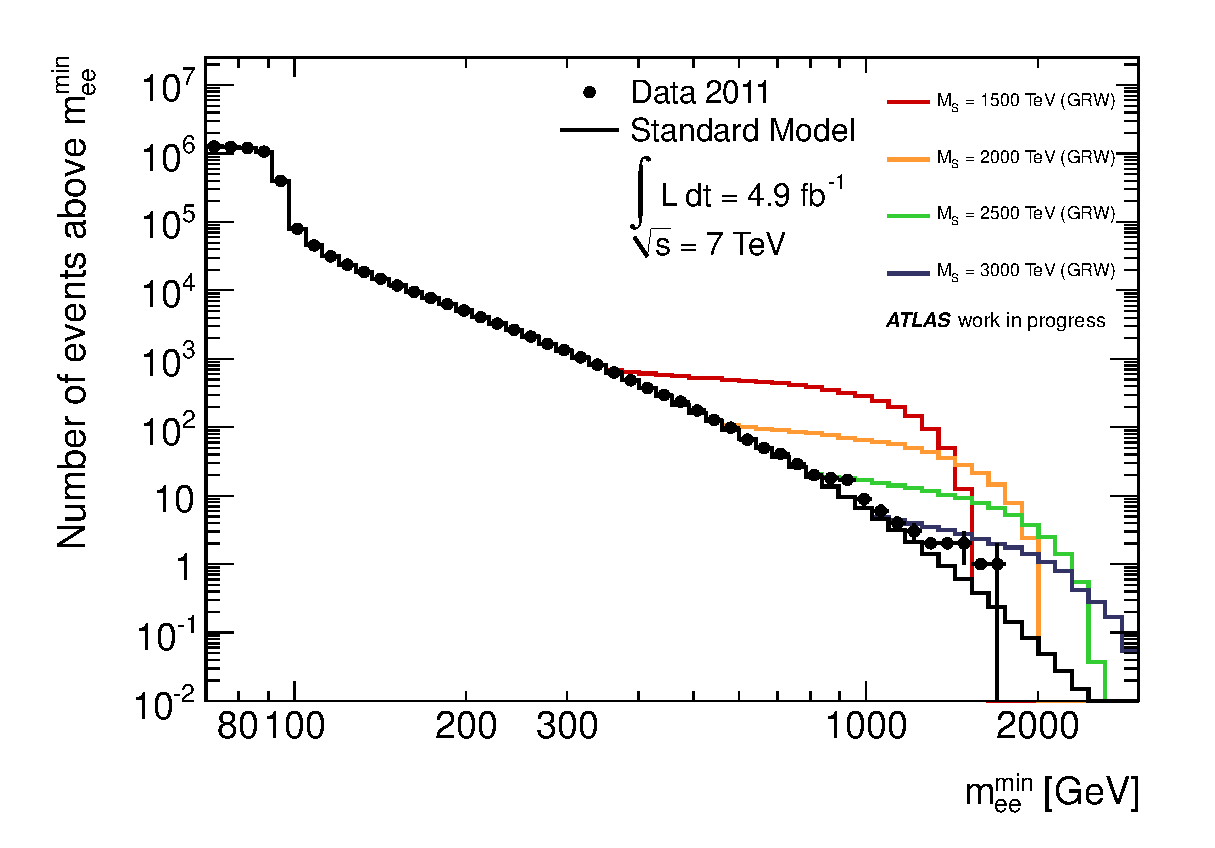
\includegraphics[width=0.9\linewidth]{images/ADD_int_inv_mass.eps}
	\caption{Dielectron intergrated invariant mass distribution for data and total backpacking Monte Carlo simulation. Lines show expected distributions for the presence of ADD.}
	\label{fig:ADDintinvMass}
	\end{figure}


	Figures \ref{fig:CIinvMass} (\ref{fig:ADDinvMass}) show the dielectron invariant mass distribution comparing data to background MC while showing the effect CI (ADD) would have on this spectrum. Figures \ref{fig:CIintinvMass} (\ref{fig:ADDintinvMass}) then show the same spectrum but with an integrated invariant mass distribution instead which indicates better general increases in the dielectron spectrum.





\section{Statistical Analysis}

	No evidence of new physics was seen in this analysis and the same procedure was carried out here as discussed in chapter \ref{ch:stat} to obtain limits on the minimum scale of new physics. This search differers as only dielectron invariant mass is used as a search variable and search bins are found at a lower invariant mass due to the lower energy and statistics of this analysis. The CI search is carried out in 5 search bins with bin edges of {110, 200, 400, 800, 1200, 3000} GeV while the ADD search was carried out in a single bin above 1300 GeV which is optimised by selecting the bin providing the highest expected limit. As in the 8 TeV analysis the expected number of events from signal was parametrised as a function of $1/\lambda^{2}$ and $1/\lambda^{4}$ for CI and $1/M_{s}^{4}$ and $1/M_{s}^{8}$ for ADD. Table \ref{tab:sys7} shows the list of systematics considered at nuisance variables for this statistical analysis. The PDFs/$\alpha_{s}$ and Weak k-factor systematics are analogous to the PDF variation systematic from the 8 TeV analysis while all others mentioned are the same. 


	\begin {table}[h]
        \begin{center}
        \begin{tabular}{ | l | c c | } 
            \hline
            Source 					& Signal            & Background         		\\
            \hline
            Normalization       	& 5.0\% ~(5.0\%)      	& NA        			\\
			PDFs/$\alpha_{s}$		& NA 			      	& 7.0\% ~(20.0\%)      	\\
			Weak k-factor       	& NA 			      	& 2.3\% ~(4.5\%)       	\\
			Efficiency  	     	& 1.0\% ~(2.0\%)      	& 1.0\% ~(2.0\%)       	\\
			Scale/Resolution       	& 1.2\% ~(2.4\%)      	& 1.2\% ~(2.4\%)       	\\
			QCD/W+jets background  	& NA 			      	& 12.0\% ~(26.0\%)      \\
            \hline  
            Total               	& 5.0\% ~(6.0\%)      	& 14.0\% ~(33.0\%)      \\
            \hline
        \end{tabular}
        \caption{Table listing all sources of systematic error and their approximate size for dielectron mass of 1 TeV (2 TeV).}
        \label{tab:sys7}
        \end{center}
    \end {table}



	As no evidence of new physics was found then a Bayesian statistical analysis was used to set a limit on $\Lambda$ and $M_{s}$. These limits can be seen in table \ref{tab:Limits7}. Expected limits were obtained by running 1000 PE's and take the mean limit in $\Lambda$ and $M_{s}$ for CI and ADD. Combined limits were also calculated with the dimuon search channel giving the highest limits on the scale of new physics for both CI and ADD at the time the paper was released.
	The Limits obtained in the 7 TeV analysis constituted the highest limits on either model when obtained  the 8 TeV results then replace them within more formalisms. Major improvements can also be seen in the upgrades to the analysis procedure between the two making the 8 TeV analysis far more mature. 


	\begin{table}[h!]
	\centering % centering table
	\begin{tabular}{l cc} % creating eight columns
	\hline\hline \\[-2ex] %inserting double-line
	Channel & ee & ee+$\mu\mu$\\  [0.2ex]
	\hline  \\[-2ex] % inserts single-line
	Expected CI constructive & 13.73 TeV & 15.10 TeV\\ 
	Expected CI destructive & 10.41 TeV & 11.42 TeV \\ 
	\hline  \\[-2ex] % inserts single-line
	Observed CI constructive & 11.60 TeV & 12.70 TeV \\ 
	Observed CI destructive & 8.76 TeV & 9.63 TeV \\ 
	\hline\hline  \\[-2ex] % inserts single-line
	Expected ADD & 2.84 TeV & 2.94 TeV \\ 
	\hline  \\[-2ex] % inserts single-line
	Observed ADD & 2.71 TeV & 2.94 TeV \\ 
	\hline\hline  \\ %[0.2ex] %inserting double-line
	\end{tabular}
	\caption{Table of 95\% confidence level limits found in the CI and ADD analyses.} %title of the table
	\label{tab:Limits7}
	\end{table}











































	% A comparison between the observed events yields and expected yield for a range of different CI benchmarks is done using 

	% \begin{equation}
	%         \mu = n_{DY+CI}(\theta,\bar{\nu}) + n_{non-DY bg}(\bar{\nu}),
	% \end{equation}

	% where $\mu$ is the number of expected events in each mass bin and n$_{DY+CI}$ and n$_{non-DY}$ are the number of events predicted by a particular benchmark signal sample and the number of predicted non DY background events respectively. $\nu$ is a set of Gaussian nuisance parameters that account for systematic uncertainties in the analysis while $\theta$ corresponds to the energy scale $\Lambda$.
	% The likelihood function for observing a set of $\bar{n}$ events in $N$ mass bins is therefore given by: 

	% \begin{equation}
	%         \mathcal{L} (\bar{n}~|~\theta,\bar{\nu}) = \prod_{k=1}^{N} \frac{ \mu_{k}^{n_{k}} e^{-\mu_{k}} }{n_{k}!}
	% \end{equation}

	% as a product of Poission probabilities for each mass bin $k$. Using Bayes' theorem this gives posterior probability

	% \begin{equation}
	%         \mathcal{P}(\theta~|~\bar{n}) = \frac{1}{\mathcal{Z}} \mathcal{L}_{M}(\bar{n}~|~\theta)P(\theta)
	% \end{equation}

	% where Z is a normalisation constant and $\mathcal{L_{M}}$ is the marginalised likelihood after all nuisance parameters have been integrated out. A prior probability for $P(\theta)$ is chosen to be flat in $1/\Lambda^{2}$, motivated by the CI differential cross-section (Eq. \ref{eq:DiffCross}).

	% A 95\% confidence level (CL) limit is found by finding $\Lambda_{lim}$ that satisfies $\int_{0} ^{\theta_{lim}} P(\theta~|~\bar{n}) d\theta = 0.95$ with $\theta = 1/\Lambda^{2}$. For this analysis the Bayesian Analysis Toolkit (BAT) \cite{BAT} was used to do this calculation. 




